\section{商谱}
\label{sec:adjacency-spectral-invariant}

完整邻接谱包含全部$n$个特征值，计算时需要处理$n\times n$矩阵。如果图中的顶点可以按连接角色分成$k$个块（$k\leq n$），使得同一块内的顶点对各个块具有完全相同的邻居计数，那么块与块之间的数值传递就可以用一个规模小得多的$k\times k$矩阵——商矩阵——来完整描述。从商矩阵算出的$k$个特征值称为图的商谱。

商谱并非对原图特征值的粗略数值近似，而是完整邻接谱中对应于“块内取常值”特征方向的精确子集。本节先定义等价划分、商矩阵与商谱，再说明颜色细化算法如何自动生成最粗的等价划分（即公平划分），最后严格证明商矩阵的实谱性质、不变子空间分解以及商谱对完整谱的精确嵌入定理。

\subsection{商矩阵}
\label{sec:adjacency-equitable-quotient}

我们先在四点环加对角边$\{1,3\}$的图上观察一种特殊的分块赋值现象。把度为$3$的两个对角顶点归为第一块$C_1=\{1,3\}$，把度为$2$的另外两个顶点归为第二块$C_2=\{2,4\}$。如图~\ref{fig:adjacency-quotient-block-values}(a)所示，给$C_1$中的顶点$1,3$统一赋读数$a$，给$C_2$中的顶点$2,4$统一赋读数$b$，构成块常值向量$\bm x=(a,b,a,b)^\top$。

现在对$\bm x$施加一次邻接矩阵$\bm A$，逐点查看邻居读数之和：在第一块$C_1$中，顶点$1$的三个邻居是$3\in C_1$（读数$a$）以及$2,4\in C_2$（读数各为$b$），邻居和为$1\cdot a+2\cdot b=a+2b$，顶点$3$的三个邻居是$1\in C_1$和$2,4\in C_2$，邻居和同样为$a+2b$。

在第二块$C_2$中，顶点$2$和顶点$4$的两个邻居都是$1,3\in C_1$（读数各为$a$）、在$C_2$内部没有邻居，故邻居和同为$2\cdot a+0\cdot b=2a$。如图~\ref{fig:adjacency-quotient-block-values}(b)所示，经过邻接矩阵作用后，同一块内的顶点依然保持相同的输出值。第一块统一从$a$更新为$a+2b$，第二块统一从$b$更新为$2a$。这意味着我们无需再逐个追踪全部$4$个顶点，只需用一个$2\times 2$小矩阵就能直接写出两块代表值$(a,b)^\top$的更新规则：
\[
\begin{bmatrix}1&2\\2&0\end{bmatrix}
\begin{bmatrix}a\\b\end{bmatrix}
=\begin{bmatrix}a+2b\\2a\end{bmatrix}.
\]

\begin{BookInlineFigure}
  \centering
  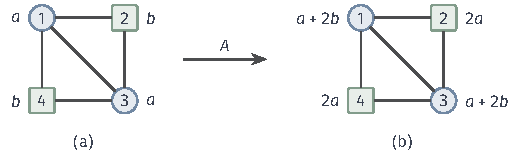
\includegraphics{figures/03-graphs/05-matrices-and-spectra/tikz/adjacency-quotient-block-values/figure.pdf}
  \caption{四点五边图上的块常值赋值与邻接更新。(a) 圆形顶点$C_1=\{1,3\}$统一赋读数$a$，方形顶点$C_2=\{2,4\}$统一赋读数$b$。(b) 经邻接矩阵$\bm A$作用后，$C_1$内每个顶点同取$a+2b$，$C_2$内每个顶点同取$2a$，输出仍为块常值向量。}
  \label{fig:adjacency-quotient-block-values}
\end{BookInlineFigure}

为什么同块内的顶点在乘$\bm A$之后还能保持取值一致？关键在于：同一个块$C_i$中的每一个顶点，落在任意块$C_j$中的邻居个数都是同一个常数。把这一结构条件提炼出来，就得到等价划分与商矩阵的定义。

\begin{definition}[等价划分与商矩阵]
\label{def:adjacency-equitable-partition}
设$\mathcal P=\{C_1,\ldots,C_r\}$是图$\mathcal G=(V,E)$顶点集$V$的一个划分（各块$C_i$非空且互不相交）。若对任意一对下标$i,j\in\{1,\ldots,r\}$（允许$i=j$），块$C_i$中的每一个顶点$u\in C_i$在块$C_j$中所拥有的邻居个数都等于同一个常数$q_{i,j}$（即$\bigl|N(u)\cap C_j\bigr|=q_{i,j}$仅依赖于$i,j$而与$u\in C_i$的具体选取无关），则称$\mathcal P$为图$\mathcal G$的一个\term{等价划分}（equitable partition）。由块间邻居计数$q_{i,j}$排成的$r\times r$矩阵$\bm Q=(q_{i,j})\in\mathbb R^{r\times r}$称为该等价划分的\term{商矩阵}（quotient matrix），$\bm Q$的全部特征值组成的多重集$\operatorname{spec}(\bm Q)$称为对应的\term{商谱}（quotient spectrum）。
\end{definition}

在上面四点五边图的划分$C_1=\{1,3\},C_2=\{2,4\}$中，$q_{1,1}=1,q_{1,2}=2,q_{2,1}=2,q_{2,2}=0$，商矩阵正是
\[
\bm Q=
\begin{bmatrix}
1&2\\
2&0
\end{bmatrix}.
\]
解二次特征方程$\det(\lambda\bm I-\bm Q)=\lambda(\lambda-1)-4=\lambda^2-\lambda-4=0$，立得商谱为
\[
\operatorname{spec}(\bm Q)=\left\{\frac{1+\sqrt{17}}{2},\;\frac{1-\sqrt{17}}{2}\right\}.
\]
原图的完整邻接谱有$4$个特征值，而商谱给出了其中$2$个——那么怎样在一般图上自动寻找这样的划分？另外$2$个特征值又藏在哪里？下面两小节依次回答这两个问题。

\subsection{公平划分}
\label{sec:adjacency-color-refinement-partition}

上一小节从分块矩阵的邻居计数定义了等价划分，但一张图往往存在不止一个等价划分（例如把每个顶点各自单独作为一块，总是包含$n$块的平凡等价划分）。在图算法中，我们希望从没有任何先验区分的统一初色出发，完全依靠图的局部连接结构自动划分出最精简的顶点类别。为此，先从顶点着色（色类）的角度给出公平划分的定义。

\begin{definition}[公平划分]
\label{def:fair-partition}
设图$\mathcal G=(V,E)$的顶点集$V$被划分为$k$个互不相交的非空子集（称为色类或单元）：
\[
V=C_1\cup C_2\cup\cdots\cup C_k.
\]
称该划分为图$\mathcal G$的一个\term{公平划分}（fair partition），如果对任意两个色类$C_i$与$C_j$（$1\leq i,j\leq k$，$i$与$j$可相同也可不同），色类$C_i$中的任意顶点$u\in C_i$在色类$C_j$中的邻居个数都等于一个固定常数$b_{i,j}=\bigl|N(u)\cap C_j\bigr|$，该常数仅取决于色类对$(C_i,C_j)$，而与顶点$u\in C_i$的具体选择无关。
\end{definition}

对比定义~\ref{def:adjacency-equitable-partition}与定义~\ref{def:fair-partition}可以看出，公平划分与等价划分所要求的块间邻居计数条件（$b_{i,j}=q_{i,j}$）在数学上完全一致。本章把这两个名称作为同义表述，不以构造方式区分它们。颜色细化的稳定划分是其中一个特殊成员，须另行证明其最粗性。下面我们依次证明：颜色细化的稳定划分必为公平划分，且它是图上所有等价划分中最粗（块数最少）的那一个。

\subsubsection{颜色细化的稳定划分}
\label{sec:adjacency-color-refinement-stable}

回顾第~\ref{sec:graph-wl-refinement}节的颜色细化算法：初始时（第$0$轮），给图中所有顶点赋同一种初始颜色；在每一轮迭代中，同时检验每个顶点当前的自身颜色以及它在各个当前色类中的邻居个数（合称为该顶点的颜色签名），只有自身颜色相同且对每种颜色的邻居个数也完全相同的顶点，才在下一轮归入同一个新色类，否则就被拆分成不同的色类。由于每次拆分都会使色类的个数严格增加，而$n$个顶点至多只能拆成$n$个单点色类，因此迭代必然在有限步（至多$n-1$轮拆分）内达到稳定状态——即再执行一轮细化，色类划分不再发生任何改变。

图~\ref{fig:adjacency-color-refinement-steps}展示了四点五边图从统一初色出发的颜色细化过程：
\begin{itemize}
\item \textbf{第$0$轮（统一初色）}：如图~\ref{fig:adjacency-color-refinement-steps}(a)所示，四个顶点$\{1,2,3,4\}$全部涂成同一种初始颜色（色$0$）。
\item \textbf{第$1$轮（按度分色）}：如图~\ref{fig:adjacency-color-refinement-steps}(b)所示，统计每个顶点在色$0$中的邻居个数（即顶点度）：顶点$1,3$各有$3$个色$0$邻居（$d=3$），顶点$2,4$各有$2$个色$0$邻居（$d=2$）。于是顶点集分裂为两个色类$C_1=\{1,3\}$（蓝圆）与$C_2=\{2,4\}$（绿方）。
\item \textbf{第$2$轮（核对邻居色分布并稳定）}：如图~\ref{fig:adjacency-color-refinement-steps}(c)所示，分别统计每个顶点在$(C_1,C_2)$两个色类中的邻居个数：$C_1$中的顶点$1$和$3$在$(C_1,C_2)$中的邻居个数同为$(1,2)$；$C_2$中的顶点$2$和$4$在$(C_1,C_2)$中的邻居个数同为$(2,0)$。同一色类内部的所有顶点具有完全相同的邻居计数签名，不再发生任何拆分，算法稳定于划分$\mathcal P_{\mathrm{stable}}=\bigl\{\{1,3\},\{2,4\}\bigr\}$。
\end{itemize}
又如在六元环$C_6$（或任意$d$正则图）上，第$0$轮所有顶点同为色$0$，第$1$轮每个顶点都有$d=2$个色$0$邻居，签名完全相同，从第一步起就不再分裂，稳定划分只有一个色类$C_1=V$。

\begin{BookInlineFigure}
  \centering
  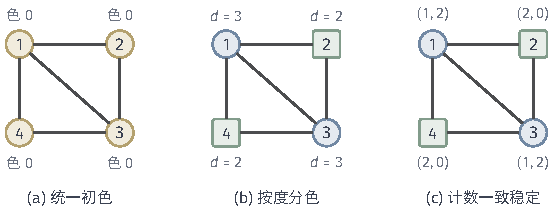
\includegraphics{figures/03-graphs/05-matrices-and-spectra/tikz/adjacency-color-refinement-steps/figure.pdf}
  \caption{四点五边图上的颜色细化稳定过程。(a) 第$0$轮：所有顶点赋统一初色（色$0$）。(b) 第$1$轮：按色$0$邻居数（即顶点度）拆分为度$3$色类$C_1=\{1,3\}$（蓝圆）与度$2$色类$C_2=\{2,4\}$（绿方）。(c) 第$2$轮：$C_1$内各点对$(C_1,C_2)$的邻居计数均为$(1,2)$，$C_2$内各点均为$(2,0)$，划分达到稳定。}
  \label{fig:adjacency-color-refinement-steps}
\end{BookInlineFigure}

下面的定理说明，颜色细化停止（稳定）的那一刻，所得的色类划分自动满足公平划分的定义。

\begin{theorem}[颜色细化的稳定划分是公平划分]
\label{thm:stable-is-equitable}
对任意有限简单无向图$\mathcal G=(V,E)$，从统一初色出发运行颜色细化算法，达到稳定时的色类划分$\mathcal P_{\mathrm{stable}}=\{C_1,\ldots,C_k\}$必为图$\mathcal G$的公平划分。
\end{theorem}

\begin{proof}
设算法在达到稳定划分$\mathcal P_{\mathrm{stable}}=\{C_1,\ldots,C_k\}$后再执行一轮核对。任取两个色类$C_i,C_j\in\mathcal P_{\mathrm{stable}}$，并任取色类$C_i$中的两个顶点$u,v\in C_i$。

因为划分$\mathcal P_{\mathrm{stable}}$已经稳定，再执行一轮颜色细化不会把同属$C_i$的顶点$u$和$v$拆入不同的新色类。根据颜色细化的更新规则，两个同色顶点$u,v$在下一轮保持同色，当且仅当它们在每一个当前色类$C_\ell$（$\ell=1,\ldots,k$）中的邻居个数都分别相等。特别地，取$\ell=j$，即有
\[
\bigl|N(u)\cap C_j\bigr|=\bigl|N(v)\cap C_j\bigr|.
\]
由于$u,v\in C_i$是任意选取的，这说明$C_i$中所有顶点在$C_j$中的邻居个数都等于同一个常数$b_{i,j}$。由定义~\ref{def:fair-partition}，$\mathcal P_{\mathrm{stable}}$是公平划分。
\end{proof}

\subsubsection{最粗等价划分}
\label{sec:adjacency-coarsest-equitable-partition}

既然公平划分与等价划分满足相同的块间邻居计数条件，为什么由颜色细化生成的公平划分在所有等价划分中地位最特殊？答案是：它合并了尽可能多的“结构角色不可区分”的顶点，是图上所有等价划分中最粗（块数最少）的那一个。为了严格表述这一结论，我们先定义两个划分之间的细化偏序关系。

\begin{definition}[划分的细化]
\label{def:partition-refinement}
设$\mathcal P=\{D_1,\ldots,D_r\}$与$\mathcal P'=\{C_1,\ldots,C_k\}$是同一顶点集$V$上的两个划分。若$\mathcal P$中的每一个块$D_a$都完整地包含在$\mathcal P'$的某一个块$C_i$之内（即对每个$a\in\{1,\ldots,r\}$，存在$i\in\{1,\ldots,k\}$使得$D_a\subseteq C_i$），则称划分$\mathcal P$是划分$\mathcal P'$的\term{细化}（refinement），或称$\mathcal P'$比$\mathcal P$更粗（coarser）。若$\mathcal P$是$\mathcal P'$的细化且$\mathcal P\neq\mathcal P'$，则称$\mathcal P$是$\mathcal P'$的严格细化。
\end{definition}

根据定义~\ref{def:partition-refinement}，说$\mathcal P$是$\mathcal P'$的细化，直观上就是指$\mathcal P$可以通过把$\mathcal P'$的某些块进一步切碎得到；等价地，$\mathcal P'$的每一个块$C_i$都恰好是$\mathcal P$中若干个完整块的并集。例如在四点集$\{1,2,3,4\}$上，$\mathcal P=\bigl\{\{1\},\{2\},\{3,4\}\bigr\}$是$\mathcal P'=\bigl\{\{1,2\},\{3,4\}\bigr\}$的细化（将$\{1,2\}$拆成了$\{1\}$和$\{2\}$）；而$\bigl\{\{1,3\},\{2,4\}\bigr\}$不是$\mathcal P'$的细化，因为块$\{1,3\}$横跨了$\mathcal P'$的两个块。在全体划分中，最细的划分是每个顶点各自成一块的单点划分（共$n$块），最粗的划分是全体顶点合成一块的整图划分（仅$1$块）。

现在我们证明：任何等价划分都是颜色细化稳定划分的细化。

\begin{theorem}[统一初色的稳定划分是最粗等价划分]
\label{thm:color-refinement-coarsest}
设$\mathcal P_{\mathrm{stable}}=\{C_1,\ldots,C_k\}$是从统一初色出发运行颜色细化得到的稳定公平划分，$\mathcal P=\{D_1,\ldots,D_r\}$是图$\mathcal G$的任意一个等价划分。则$\mathcal P$必为$\mathcal P_{\mathrm{stable}}$的细化（即$\mathcal P_{\mathrm{stable}}$是图$\mathcal G$最粗的等价划分，并在不计块的排列次序下唯一确定）。
\end{theorem}

\begin{proof}
记$\mathcal P^{(t)}$为颜色细化第$t$轮结束时的色类划分（$t=0,1,2,\ldots$）。我们对轮数$t$作数学归纳法，证明对一切$t\geq 0$，$\mathcal P$都是$\mathcal P^{(t)}$的细化——即颜色细化在任何一轮都不会把等价划分$\mathcal P$的同一个块$D_a$中的两个顶点拆开。

\textbf{归纳基础（$t=0$）}：第$0$轮为统一初色，$\mathcal P^{(0)}=\{V\}$只有一个块。对任意$D_a\in\mathcal P$，显然有$D_a\subseteq V$，故$\mathcal P$是$\mathcal P^{(0)}$的细化。

\textbf{归纳步骤}：假设第$t$轮结束时$\mathcal P$是$\mathcal P^{(t)}$的细化。这意味着$\mathcal P^{(t)}$中的每一个当前色类$C\in\mathcal P^{(t)}$，都恰好是$\mathcal P$中若干个完整块的并集。

现在考察第$t+1$轮的颜色更新。任取$\mathcal P$的一个块$D_a\in\mathcal P$，并任取其中的两个顶点$u,v\in D_a$。由归纳假设，$u$和$v$在第$t$轮属于同一个色类，具有相同的第$t$轮颜色。要证明它们在第$t+1$轮仍然获得相同颜色，只需证明对$\mathcal P^{(t)}$中的任意一个色类$C\in\mathcal P^{(t)}$，$u$和$v$在$C$中的邻居个数相等。

由于$C\in\mathcal P^{(t)}$是$\mathcal P$中若干个互不相交块的并集，设
\[
C=D_{b_1}\cup D_{b_2}\cup\cdots\cup D_{b_s}.
\]
因为$\mathcal P=\{D_1,\ldots,D_r\}$是等价划分（商矩阵记为$q_{a,b}$），块$D_a$中的任意顶点在块$D_{b_\ell}$中的邻居个数都等于固定常数$q_{a,b_\ell}$。由于$D_{b_1},\ldots,D_{b_s}$互不相交，顶点$u\in D_a$在并集$C$中的邻居总数为
\[
\bigl|N(u)\cap C\bigr|
=\sum_{\ell=1}^s\bigl|N(u)\cap D_{b_\ell}\bigr|
=q_{a,b_1}+q_{a,b_2}+\cdots+q_{a,b_s}.
\]
完全相同地，顶点$v\in D_a$在$C$中的邻居总数也为
\[
\bigl|N(v)\cap C\bigr|
=\sum_{\ell=1}^s\bigl|N(v)\cap D_{b_\ell}\bigr|
=q_{a,b_1}+q_{a,b_2}+\cdots+q_{a,b_s}
=\bigl|N(u)\cap C\bigr|.
\]
这对所有色类$C\in\mathcal P^{(t)}$均成立，故$u$和$v$在第$t+1$轮的颜色签名完全一致，仍然留在同一个第$t+1$轮色类中。因此，块$D_a$的全体顶点整体包含在$\mathcal P^{(t+1)}$的某个色类中，即$\mathcal P$也是$\mathcal P^{(t+1)}$的细化。

由数学归纳法，当算法在有限步达到稳定划分$\mathcal P_{\mathrm{stable}}$时，$\mathcal P$仍是$\mathcal P_{\mathrm{stable}}$的细化。
\end{proof}

定理~\ref{thm:color-refinement-coarsest}给出了一个构造结论：我们不需要靠人工猜测去寻找等价划分，只需从统一初色运行确定性的颜色细化算法，就一定能找到全图最粗、块数最少（从而商矩阵维数最小）的规范公平划分$\mathcal P_{\mathrm{stable}}$。当需要判断两张图$\mathcal G$和$\mathcal H$是否可能同构时，可以在它们的不交并$\mathcal G\sqcup\mathcal H$上使用同一套颜色编码同步运行颜色细化：若两图同构，稳定后每个色类在两图中的顶点数$|C_i|$以及块间邻居计数$b_{i,j}$必定完全匹配，导出相同的公平划分商矩阵$\bm Q$；反之，只要色类大小或商矩阵不匹配，立即可断定两图不同构。

\subsection{公平划分的性质}
\label{sec:adjacency-spectral-hierarchy}

找到公平划分$\mathcal P=\{C_1,\ldots,C_k\}$及其$k\times k$商矩阵$\bm Q=(b_{i,j})$之后，一个核心的谱图论问题是：这个小矩阵$\bm Q$的特征值（商谱）与原图$n\times n$邻接矩阵$\bm A$的特征值（完整邻接谱）之间究竟有什么关系？下面我们分三个子小节，通过形式化定理和严格证明逐一揭示商矩阵的实谱性质、块常值不变子空间交织恒等式以及商谱对完整谱的精确嵌入分解，并剖析商谱保留与丢失的结构信息。

\subsubsection{商矩阵的实谱}
\label{sec:adjacency-quotient-real-spectrum}

首先，对给定的图$\mathcal G$，一般的等价划分可以有很多个，各自导出不同阶数的商矩阵；但根据定理~\ref{thm:color-refinement-coarsest}，从统一初色出发由颜色细化生成的公平划分$\mathcal P=\{C_1,\ldots,C_k\}$作为最粗等价划分是唯一确定的。因此，在不计$k$个色类排列顺序（即对$\bm Q$的行和列同时施加相同置换$\bm P\bm Q\bm P^\top$）的意义下，公平划分导出的商矩阵$\bm Q$及其商谱$\operatorname{spec}(\bm Q)$是图$\mathcal G$唯一确定的代数不变量。

其次，观察商矩阵$\bm Q=(b_{i,j})$的形式：虽然原图的邻接矩阵$\bm A$是对称矩阵，但商矩阵$\bm Q$通常不是对称矩阵。例如在三点路径$1\text{--}2\text{--}3$上，公平划分将两个度为$1$的端点归为第一块$C_1=\{1,3\}$（$|C_1|=2$），将度为$2$的中心点归为第二块$C_2=\{2\}$（$|C_2|=1$）。此时，$C_1$中的每个端点在$C_2$中只有$b_{1,2}=1$个邻居，而$C_2$中的中心点在$C_1$中却有$b_{2,1}=2$个邻居，商矩阵为
\[
\bm Q=\begin{bmatrix}0&1\\2&0\end{bmatrix},\qquad b_{1,2}=1\neq 2=b_{2,1}.
\]
既然$\bm Q$不对称，它的特征值会不会出现复数？能不能对角化？下面的定理通过“双向计数跨块边数”证明：商矩阵$\bm Q$虽然自身未必对称，但通过块大小对角矩阵作一次对角相似变换，就能变成实对称矩阵。

\begin{theorem}[商矩阵的实谱性质]
\label{thm:quotient-matrix-real-spectrum}
设$\mathcal P=\{C_1,\ldots,C_k\}$是有限简单无向图$\mathcal G=(V,E)$的一个公平划分（或任意等价划分），商矩阵为$\bm Q=(b_{i,j})\in\mathbb R^{k\times k}$，记块大小对角矩阵为
\[
\bm D_C=\operatorname{diag}\bigl(|C_1|,|C_2|,\ldots,|C_k|\bigr).
\]
则块大小与商矩阵满足对称平衡恒等式
\begin{equation}
|C_i|\,b_{i,j}=|C_j|\,b_{j,i}\quad(\forall\,1\leq i,j\leq k),
\qquad\text{即}\qquad
\bm D_C\bm Q=\bm Q^\top\bm D_C.
\label{eq:adjacency-quotient-symmetry}
\end{equation}
进一步，矩阵
\[
\widetilde{\bm Q}=\bm D_C^{1/2}\bm Q\bm D_C^{-1/2}
\]
是$k\times k$实对称矩阵。因此，商矩阵$\bm Q$在实数域$\mathbb R$上可对角化，其全部$k$个特征值均为实数。
\end{theorem}

\begin{proof}
任取两个色类$C_i$与$C_j$（当$i=j$时$|C_i|b_{i,i}=|C_j|b_{j,i}$恒成立；以下设$i\neq j$），我们从左右两侧分别计算横跨在$C_i$与$C_j$之间的无向边总数$e(C_i,C_j)$：从$C_i$一侧计数，$C_i$中共有$|C_i|$个顶点，由公平划分定义，其中每一个顶点在$C_j$中都恰好有$b_{i,j}$个邻居，故跨块边总数为$e(C_i,C_j)=|C_i|\,b_{i,j}$；从$C_j$一侧计数，$C_j$中共有$|C_j|$个顶点，其中每一个顶点在$C_i$中都恰好有$b_{j,i}$个邻居，故同一批跨块边的总数又等于$e(C_i,C_j)=|C_j|\,b_{j,i}$。两边相等即得$|C_i|\,b_{i,j}=|C_j|\,b_{j,i}$。注意到$(\bm D_C\bm Q)_{i,j}=|C_i|b_{i,j}$，而$(\bm Q^\top\bm D_C)_{i,j}=(\bm Q^\top)_{i,j}|C_j|=b_{j,i}|C_j|$，故矩阵等式$\bm D_C\bm Q=\bm Q^\top\bm D_C$成立，式~\eqref{eq:adjacency-quotient-symmetry}得证。

由于每个色类$C_i$非空，$|C_i|\geq 1>0$，对角矩阵
\[
\bm D_C^{1/2}=\operatorname{diag}\bigl(\sqrt{|C_1|},\ldots,\sqrt{|C_k|}\bigr)
\]
及其逆矩阵$\bm D_C^{-1/2}$均为实可逆对角矩阵。对$\bm D_C\bm Q=\bm Q^\top\bm D_C$两端左乘$\bm D_C^{-1/2}$、右乘$\bm D_C^{-1/2}$，得到
\[
\bm D_C^{1/2}\bm Q\bm D_C^{-1/2}
=\bm D_C^{-1/2}\bm Q^\top\bm D_C^{1/2}
=\bigl(\bm D_C^{1/2}\bm Q\bm D_C^{-1/2}\bigr)^\top,
\]
这证明了$\widetilde{\bm Q}=\bm D_C^{1/2}\bm Q\bm D_C^{-1/2}$是实对称矩阵（其第$(i,j)$个元素为$b_{i,j}\sqrt{|C_i|/|C_j|}=b_{j,i}\sqrt{|C_j|/|C_i|}$）。

由实对称矩阵谱定理，$\widetilde{\bm Q}$有$k$个实特征值和一组标准正交实特征向量基$\tilde{\bm y}_1,\ldots,\tilde{\bm y}_k$。因为$\bm Q=\bm D_C^{-1/2}\widetilde{\bm Q}\bm D_C^{1/2}$与实对称矩阵$\widetilde{\bm Q}$相似，二者具有完全相同的特征多项式与实特征值，且$\bm y_r=\bm D_C^{-1/2}\tilde{\bm y}_r$（$r=1,\ldots,k$）构成$\bm Q$在$\mathbb R^k$中的一组线性无关实特征向量基，故$\bm Q$在$\mathbb R$上可对角化。
\end{proof}

\subsubsection{商谱嵌入}
\label{sec:adjacency-quotient-spectrum-embedding}

为了把$k\times k$商矩阵$\bm Q$与$n\times n$邻接矩阵$\bm A$连接起来，我们引入公平划分$\mathcal P=\{C_1,\ldots,C_k\}$的\emph{块指示矩阵}（characteristic matrix）$\bm S\in\mathbb R^{n\times k}$：其第$j$列就是色类$C_j$在顶点空间$\mathbb R^n$中的$0$--$1$指示向量$\bm 1_{C_j}$：
\[
S_{u,j}=(\bm 1_{C_j})_u=
\begin{cases}
1,& u\in C_j,\\
0,& u\notin C_j,
\end{cases}
\qquad 1\leq u\leq n,\;1\leq j\leq k.
\]
由于$C_1,\ldots,C_k$互不相交且非空，$\bm S$的各列在不同坐标集合上取$1$，满足
\[
\bm S^\top\bm S=\operatorname{diag}\bigl(|C_1|,\ldots,|C_k|\bigr)=\bm D_C,
\]
故$\bm S$列满秩（$\operatorname{rank}\bm S=k$）。

对任意块读数向量$\bm y=(y_1,\ldots,y_k)^\top\in\mathbb R^k$，左乘$\bm S$得到的$n$维向量
\[
\bm S\bm y=\sum_{j=1}^k y_j\,\bm 1_{C_j}\in\mathbb R^n
\]
在每个色类$C_j$的所有顶点上统一取常数值$y_j$。因此，$\bm S$的列空间
\[
\mathcal W=\operatorname{col}(\bm S)=\bigl\{\bm S\bm y:\bm y\in\mathbb R^k\bigr\}\subseteq\mathbb R^n
\]
是由全体“在每个色类内部取常值”的顶点向量组成的$k$维子空间，称为划分$\mathcal P$的\term{块常值子空间}（block-constant subspace）。而$\mathcal W$在$\mathbb R^n$中的正交补空间
\[
\mathcal W^\perp
=\ker(\bm S^\top)
=\Bigl\{\bm z\in\mathbb R^n:\bm 1_{C_j}^\top\bm z=\sum_{u\in C_j}z_u=0,\;\forall\,j=1,\ldots,k\Bigr\}
\]
则由全体“在每一个色类内部分量之和均为零”的顶点向量组成，维数为$n-k$。

下面的定理揭示了公平划分的本质代数特征：块常值子空间$\mathcal W$及其正交补$\mathcal W^\perp$都是邻接矩阵$\bm A$的不变子空间。

\begin{theorem}[商矩阵的交织恒等式]
\label{thm:quotient-intertwining}
设$\mathcal P=\{C_1,\ldots,C_k\}$是图$\mathcal G=(V,E)$的顶点集划分，$\bm S\in\mathbb R^{n\times k}$为其块指示矩阵。则$\mathcal P$是以$\bm Q=(b_{i,j})\in\mathbb R^{k\times k}$为商矩阵的公平划分（等价划分），当且仅当邻接矩阵$\bm A$与商矩阵$\bm Q$满足交织恒等式
\begin{equation}
\bm A\bm S=\bm S\bm Q.
\label{eq:adjacency-quotient-intertwining}
\end{equation}
在此条件下，块常值子空间$\mathcal W=\operatorname{col}(\bm S)$及其正交补空间$\mathcal W^\perp=\ker(\bm S^\top)$均为$\bm A$的不变子空间（即$\bm A\mathcal W\subseteq\mathcal W$且$\bm A\mathcal W^\perp\subseteq\mathcal W^\perp$）。
\end{theorem}

\begin{proof}
首先证明$\mathcal P$为商矩阵是$\bm Q$的公平划分当且仅当$\bm A\bm S=\bm S\bm Q$。任取顶点$u\in V$（设$u$属于色类$C_i$）和列下标$j\in\{1,\ldots,k\}$，分别计算式~\eqref{eq:adjacency-quotient-intertwining}左右两端在位置$(u,j)$处的元素。左端$\bm A\bm S$的第$j$列为$\bm A\bm 1_{C_j}$，其在顶点$u$处的元素为
\[
(\bm A\bm S)_{u,j}=(\bm A\bm 1_{C_j})_u=\sum_{v\in C_j}a_{u,v}=\bigl|N(u)\cap C_j\bigr|,
\]
即顶点$u$在色类$C_j$中的邻居个数；右端$\bm S\bm Q$在位置$(u,j)$处的元素为$\sum_{\ell=1}^k S_{u,\ell}\,b_{\ell,j}$，因为$u\in C_i$，只有$\ell=i$时$S_{u,i}=1$、其余$\ell\neq i$时$S_{u,\ell}=0$，故
\[
(\bm S\bm Q)_{u,j}=b_{i,j}.
\]
对比左右两端可知：$(\bm A\bm S)_{u,j}=(\bm S\bm Q)_{u,j}$对所有$u\in C_i$和所有$i,j$成立，当且仅当对任意$u\in C_i$都有$|N(u)\cap C_j|=b_{i,j}$，这正是定义~\ref{def:fair-partition}中公平划分的充要条件。

接下来证明$\mathcal W$与$\mathcal W^\perp$均为$\bm A$的不变子空间。一方面，对任意块常值向量$\bm w=\bm S\bm y\in\mathcal W$（$\bm y\in\mathbb R^k$），由交织恒等式~\eqref{eq:adjacency-quotient-intertwining}，有
\[
\bm A\bm w=\bm A(\bm S\bm y)=(\bm A\bm S)\bm y=\bm S(\bm Q\bm y)\in\operatorname{col}(\bm S)=\mathcal W,
\]
故$\bm A\mathcal W\subseteq\mathcal W$。另一方面，对任意$\bm z\in\mathcal W^\perp$和任意$\bm w\in\mathcal W$，由于$\bm A$是实对称矩阵（$\bm A^\top=\bm A$）且已证$\bm A\bm w\in\mathcal W$，有
\[
\langle\bm A\bm z,\bm w\rangle
=(\bm A\bm z)^\top\bm w
=\bm z^\top(\bm A\bm w)
=\langle\bm z,\bm A\bm w\rangle=0.
\]
这说明$\bm A\bm z$与$\mathcal W$中的一切向量正交，即$\bm A\bm z\in\mathcal W^\perp$，故$\bm A\mathcal W^\perp\subseteq\mathcal W^\perp$。定理得证。
\end{proof}

由定理~\ref{thm:quotient-intertwining}的交织恒等式$\bm A\bm S=\bm S\bm Q$，我们可以立即导出商谱与原图完整邻接谱之间的精确嵌合定理。

\begin{theorem}[商谱嵌入定理]
\label{thm:quotient-spectrum-inclusion}
设$\mathcal P=\{C_1,\ldots,C_k\}$是有限简单无向图$\mathcal G=(V,E)$的一个公平划分（或任意等价划分），块指示矩阵为$\bm S\in\mathbb R^{n\times k}$，商矩阵为$\bm Q\in\mathbb R^{k\times k}$。则：
\begin{enumerate}
\item 若$\bm y\in\mathbb R^k\setminus\{\bm 0\}$是商矩阵$\bm Q$属于特征值$\lambda$的特征向量（$\bm Q\bm y=\lambda\bm y$），则块常值向量$\bm S\bm y\in\mathcal W\setminus\{\bm 0\}$是原图邻接矩阵$\bm A$属于同一特征值$\lambda$的特征向量；
\item 按代数重数计，商矩阵的商谱$\operatorname{spec}(\bm Q)$等于$\bm A$限制在块常值子空间$\mathcal W$上的特征值多重集$\operatorname{spec}(\bm A|_{\mathcal W})$，从而完整包含在原图邻接谱中：
\[
\operatorname{spec}(\bm Q)\subseteq\operatorname{spec}(\bm A),\qquad
\operatorname{spec}(\bm A)=\operatorname{spec}(\bm Q)\,\cup\,\operatorname{spec}(\bm A|_{\mathcal W^\perp}),
\]
其中$\bm A$限制在正交补$\mathcal W^\perp$上的$n-k$个特征值$\operatorname{spec}(\bm A|_{\mathcal W^\perp})$称为该划分下的\term{剩余谱}（residual spectrum）；
\item 原图的最大邻接特征值$\lambda_1(\bm A)$必然包含在商谱$\operatorname{spec}(\bm Q)$中。
\end{enumerate}
\end{theorem}

\begin{proof}
\textbf{第1条与第2条}：因为$\bm S^\top\bm S=\bm D_C$可逆，线性映射$\bm S\colon\mathbb R^k\to\mathcal W$是双射（线性同构）：当$\bm y\neq\bm 0$时必有$\bm S\bm y\neq\bm 0$。若$\bm Q\bm y=\lambda\bm y$，由定理~\ref{thm:quotient-intertwining}的$\bm A\bm S=\bm S\bm Q$，立得
\[
\bm A(\bm S\bm y)=\bm S(\bm Q\bm y)=\bm S(\lambda\bm y)=\lambda(\bm S\bm y),
\]
即$\bm S\bm y\in\mathcal W$是$\bm A$属于特征值$\lambda$的特征向量。更进一步，式~\eqref{eq:adjacency-quotient-intertwining}表明线性算子$\bm A|_{\mathcal W}\colon\mathcal W\to\mathcal W$在基$\{\bm 1_{C_1},\ldots,\bm 1_{C_k}\}$下的表示矩阵恰好就是$\bm Q$，因此$\bm A|_{\mathcal W}$的特征多项式与$\bm Q$的特征多项式恒同，$\operatorname{spec}(\bm A|_{\mathcal W})=\operatorname{spec}(\bm Q)$（含重数）。又因$\mathbb R^n=\mathcal W\oplus\mathcal W^\perp$是$\bm A$的两个正交不变子空间的直和，在由$\mathcal W$的一组正交特征基与$\mathcal W^\perp$的一组正交特征基拼成的全空间正交基下，$\bm A$呈分块对角形$\operatorname{diag}(\bm A|_{\mathcal W},\bm A|_{\mathcal W^\perp})$，故完整邻接谱$\operatorname{spec}(\bm A)$等于商谱$\operatorname{spec}(\bm Q)$与剩余谱$\operatorname{spec}(\bm A|_{\mathcal W^\perp})$的并集。

\textbf{第3条（$\lambda_1(\bm A)\in\operatorname{spec}(\bm Q)$）}：由定理~\ref{thm:quotient-matrix-real-spectrum}，实对称矩阵$\widetilde{\bm Q}=\bm D_C^{1/2}\bm Q\bm D_C^{-1/2}$逐元素非负，与$\bm Q$（从而与$\bm A|_{\mathcal W}$）具有相同的最大特征值$\mu_{\max}=\lambda_1(\bm Q)$。在原图$\mathcal G$中取一个达到全图最大邻接特征值$\lambda_1(\bm A)$的连通分量$V_0$；当$V_0$至少含两个顶点时应用定理~\ref{thm:adjacency-perron}，单点分量则直接取其指示向量。由此存在一个在$V_0$上各分量严格为正、在$V\setminus V_0$上为$0$的非负特征向量$\bm p\in\mathbb R^n$，满足$\bm A\bm p=\lambda_1(\bm A)\bm p$。

而在正交补$\mathcal W^\perp$中，任意向量$\bm z\in\mathcal W^\perp$在每个色类$C_j$内的分量之和均为零（$\sum_{u\in C_j}z_u=0$）。考察$\bm p$在块常值子空间$\mathcal W$上的正交投影$\bm p_{\mathcal W}$：它在每个色类$C_j$上取该块内$\bm p$分量的平均值$\bar p_j=\frac{1}{|C_j|}\sum_{u\in C_j}p_u\geq 0$。因为$\bm p$在$V_0$上严格为正，至少有一个色类的平均值$\bar p_j>0$，故$\bm p_{\mathcal W}\neq\bm 0$。又因为$\mathcal W$与$\mathcal W^\perp$是$\bm A$的正交不变子空间，$\bm A\bm p=\lambda_1(\bm A)\bm p$两边向$\mathcal W$作正交投影即得$\bm A\bm p_{\mathcal W}=\lambda_1(\bm A)\bm p_{\mathcal W}$。这证明了$\bm p_{\mathcal W}\in\mathcal W\setminus\{\bm 0\}$是$\bm A|_{\mathcal W}$属于$\lambda_1(\bm A)$的特征向量，故$\lambda_1(\bm A)\in\operatorname{spec}(\bm A|_{\mathcal W})=\operatorname{spec}(\bm Q)$。
\end{proof}

我们回到四点五边图（图~\ref{fig:adjacency-quotient-block-values}），用定理~\ref{thm:quotient-spectrum-inclusion}把它的$4$个特征值完整拆解为商谱与剩余谱两部分。首先，在块常值子空间$\mathcal W$中（$k=2$个特征值），公平划分为$C_1=\{1,3\},C_2=\{2,4\}$，$\mathcal W=\operatorname{span}\{(1,0,1,0)^\top,(0,1,0,1)^\top\}$是二维的，前面已由$2\times 2$商矩阵$\bm Q=\bigl[\begin{smallmatrix}1&2\\2&0\end{smallmatrix}\bigr]$算出两个商特征值
\[
\lambda_1=\frac{1+\sqrt{17}}{2}\approx 2.562,\qquad
\lambda_4=\frac{1-\sqrt{17}}{2}\approx -1.562,
\]
全图的最大特征值$\lambda_1=(1+\sqrt{17})/2$确实落在了商谱中。

其次，在正交补$\mathcal W^\perp$中（$n-k=2$个剩余特征值），向量要求在$C_1=\{1,3\}$内分量之和为零（$z_1+z_3=0$）且在$C_2=\{2,4\}$内分量之和也为零（$z_2+z_4=0$），因此$\mathcal W^\perp$直接由两个块内反对称差向量张成：
\[
\bm z_1=(1,0,-1,0)^\top,\qquad
\bm z_2=(0,1,0,-1)^\top.
\]
将邻接矩阵$\bm A$分别作用在这两个向量上：对$\bm z_1=(1,0,-1,0)^\top$，顶点$1$读到邻居$3$的$-1$，顶点$3$读到邻居$1$的$+1$，顶点$2,4$同时读到邻居$1$的$+1$与邻居$3$的$-1$（相加为$0$），故$\bm A\bm z_1=(-1,0,1,0)^\top=-\bm z_1$，直接给出第一个剩余特征值$\lambda_3=-1$；对$\bm z_2=(0,1,0,-1)^\top$，顶点$1$和$3$各自同时连接邻居$2$（读数$+1$）和邻居$4$（读数$-1$），正负抵消为$0$，顶点$2$和$4$只连接读数为$0$的顶点$1,3$，邻居和也为$0$，故$\bm A\bm z_2=\bm 0=0\cdot\bm z_2$，给出第二个剩余特征值$\lambda_2=0$。将商谱$\bigl\{\frac{1+\sqrt{17}}{2},\frac{1-\sqrt{17}}{2}\bigr\}$与剩余谱$\{0,-1\}$合并，就精确得到了四点五边图的全部$4$个邻接特征值：
\[
\operatorname{spec}(\bm A)=\left\{\frac{1+\sqrt{17}}{2},\;0,\;-1,\;\frac{1-\sqrt{17}}{2}\right\}.
\]

\subsubsection{商谱的局限}
\label{sec:adjacency-quotient-information}

定理~\ref{thm:quotient-spectrum-inclusion}的正交分解$\mathbb R^n=\mathcal W\oplus\mathcal W^\perp$揭示了商矩阵$\bm Q$与商谱$\operatorname{spec}(\bm Q)$能够捕捉什么、又会遗漏什么。根据定义~\ref{def:fair-partition}，商矩阵$\bm Q=(b_{i,j})$只记录色类$C_i$中的每个顶点落在色类$C_j$中的邻居个数$b_{i,j}$。只要块间与块内的邻居计数$b_{i,j}$给定，邻接矩阵$\bm A$在块常值子空间$\mathcal W$上的作用就完全固定，从而唯一决定了包括全图最大特征值$\lambda_1(\bm A)$在内的全部$k$个商特征值。

然而，给定每个顶点在同色类内部的邻居个数$b_{i,i}$（或两个色类之间的邻居个数$b_{i,j}$），并不能唯一决定这些边在色类内部究竟是如何连接的。例如在一个包含$6$个顶点的色类中，要求每个顶点恰好有$b_{1,1}=2$个同色邻居，这$6$个顶点既可以首尾相连围成一个连通的六元环$C_6$，也可以拆成两个互不相连的三角形$2C_3=C_3\sqcup C_3$。任何保持各块邻居计数$b_{i,j}$不变的内部重连，都不会改变公平划分和商矩阵$\bm Q$；它们对邻接矩阵$\bm A$的影响完全局限在块内零和的正交补空间$\mathcal W^\perp$上，只可能改变该子空间上的限制算子及其剩余谱，商谱保持不变；不同限制算子仍可能同谱。

图~\ref{fig:adjacency-c6-vs-2c3-quotient}具体展示了六点环$C_6$与两个不相交三角形$2C_3$的这一对比。由于两张图都是$6$个顶点的$2$正则图，从统一初色出发运行颜色细化时，每个顶点都有$2$个同色邻居，第一轮就不发生任何分裂，稳定后的公平划分都只有$k=1$个色类$C_1=V$，导出的$1\times 1$商矩阵同为$\bm Q=(2)$，商谱同为$\operatorname{spec}(\bm Q)=\{2\}$（对应一维常向量子空间$\mathcal W=\operatorname{span}\{\bm 1\}$）。

但在五维正交补空间$\mathcal W^\perp=\bm 1^\perp$上，两张图的内部连接差异使剩余谱完全不同：连通六元环$C_6$的完整邻接谱为$\{2,1,1,-1,-1,-2\}$，扣去商谱$\{2\}$后的$5$个剩余特征值为$1,1,-1,-1,-2$。

而不连通图$2C_3$由两个三角形拼成，完整邻接谱为$\{2,2,-1,-1,-1,-1\}$，其$5$个剩余特征值为$2,-1,-1,-1,-1$（其中落在$\mathcal W^\perp$中的第二个特征值$2$直接反映了两个连通分量的存在，而这一信息在缩减为商矩阵$\bm Q=(2)$时已经丢失）。

\begin{BookInlineFigure}
  \centering
  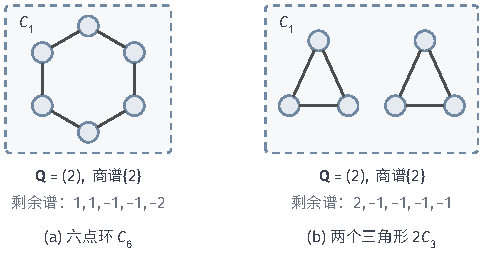
\includegraphics{figures/03-graphs/05-matrices-and-spectra/tikz/adjacency-c6-vs-2c3-quotient/figure.pdf}
  \caption{商谱相同而剩余谱不同的两张$6$点$2$正则图。在统一初色下，两图的公平划分都只有单一色类$C_1=V$（虚线框，$k=1$），商矩阵均为$\bm Q=(2)$，商谱均为$\{2\}$。(a) 六点环$C_6$在$\mathcal W^\perp$上的$5$个剩余特征值为$1,1,-1,-1,-2$。(b) 两个三角形$2C_3$在$\mathcal W^\perp$上的$5$个剩余特征值为$2,-1,-1,-1,-1$。}
  \label{fig:adjacency-c6-vs-2c3-quotient}
\end{BookInlineFigure}

最后，把$C_6$与$2C_3$的例子同第~\ref{sec:adjacency-cospectral-graphs}小节的五顶点同谱图$K_{1,4}$与$C_4\sqcup K_1$（图~\ref{fig:adjacency-cospectral-pair}）放在一起，就能看清颜色细化（公平划分）与完整邻接谱在区分非同构图时的互补关系。

一方面，商谱只是完整邻接谱在$\mathcal W$上的子集：像$C_6$与$2C_3$这样颜色细化完全无法区分（公平划分与商谱均相同）的两张正则图，仍有可能依靠$\mathcal W^\perp$上的剩余谱被完整邻接谱区分开。

另一方面，完整邻接谱也并不能涵盖颜色细化的全部信息：$K_{1,4}$与$C_4\sqcup K_1$拥有完全相同的完整邻接谱$\{2,0,0,0,-2\}$，但颜色细化在第一轮按顶点度分色时，就会把$K_{1,4}$拆成度为$4$和度为$1$的两个色类（大小$1+4$，商矩阵$\bigl(\begin{smallmatrix}0&4\\1&0\end{smallmatrix}\bigr)$），而把$C_4\sqcup K_1$拆成度为$2$和度为$0$的两个色类（大小$4+1$，商矩阵$\bigl(\begin{smallmatrix}2&0\\0&0\end{smallmatrix}\bigr)$），从而将这两张同谱图区分开。完整邻接谱与公平划分各自从特征值多重集和局部度传递层次刻画了图的结构。
